\documentclass[UTF8,zihao=-4]{ctexart}

\usepackage[a4paper,margin=2.35cm]{geometry}
\usepackage{amsmath,amssymb,amsthm,bm}
\usepackage{graphicx}
\usepackage{booktabs,longtable,array,multirow,tabularx}
\usepackage{enumitem}
\usepackage{xcolor}
\usepackage{hyperref}
\usepackage{tikz}
\usepackage{caption}
\usepackage{subcaption}
\usepackage{listings}
\usepackage{float}
\usepackage{fancyhdr}
\usepackage{titlesec}
\usetikzlibrary{arrows.meta,positioning,calc,fit,shapes.geometric}

\hypersetup{
  colorlinks=true,
  linkcolor=blue!55!black,
  citecolor=blue!55!black,
  urlcolor=blue!55!black,
  pdftitle={QPP-inspired Few-Qubit QNN for Corner and Junction Detection},
  pdfauthor={Hackathon QML project draft}
}

\pagestyle{fancy}
\fancyhf{}
\lhead{QPP-inspired Few-Qubit QNN for Corner/Junction Detection}
\rhead{\thepage}
\setlength{\headheight}{15pt}

\titleformat{\section}{\Large\bfseries}{\thesection}{0.8em}{}
\titleformat{\subsection}{\large\bfseries}{\thesubsection}{0.8em}{}
\titleformat{\subsubsection}{\normalsize\bfseries}{\thesubsubsection}{0.8em}{}

\definecolor{codebg}{RGB}{247,247,247}
\definecolor{notecolor}{RGB}{245,248,255}
\definecolor{warncolor}{RGB}{255,248,235}
\definecolor{darkgreen}{RGB}{20,110,70}
\definecolor{darkred}{RGB}{165,50,40}

\lstset{
  basicstyle=\ttfamily\small,
  backgroundcolor=\color{codebg},
  frame=single,
  framerule=0.2pt,
  rulecolor=\color{black!25},
  breaklines=true,
  columns=fullflexible,
  keepspaces=true,
  showstringspaces=false,
  tabsize=2
}

\newcommand{\Rx}{R_x}
\newcommand{\Ry}{R_y}
\newcommand{\Rz}{R_z}
\newcommand{\E}{\mathbb{E}}
\newcommand{\Tr}{\operatorname{Tr}}
\newcommand{\diag}{\operatorname{diag}}
\newcommand{\sigmoid}{\operatorname{sigmoid}}
\newcommand{\clip}{\operatorname{clip}}
\newcommand{\softplus}{\operatorname{softplus}}
\newcommand{\zz}{\langle Z_0Z_1\rangle}
\newcommand{\zzero}{\langle Z_0\rangle}
\newcommand{\zone}{\langle Z_1\rangle}

\newtheorem{theorem}{定理}
\newtheorem{proposition}{命题}
\newtheorem{remark}{备注}

\newenvironment{note}{\begin{quote}\small\noindent\textbf{说明：}}{\end{quote}}
\newenvironment{warningbox}{\begin{quote}\small\noindent\textbf{注意：}}{\end{quote}}

\title{\bfseries 面向角点/交叉点检测的 QPP-inspired Few-Qubit QNN 计划书\\[0.35em]
\large 从单量子比特解析函数逼近到二维局部结构特征分类}
\author{短期 Quantum Hackathon 项目草案}
\date{2026 年 6 月 27 日}

\begin{document}
\maketitle

\begin{abstract}
本文提出一个面向图像角点、交叉点与关键点检测的短期 QML 项目方案。核心思想不是将整张图像直接输入量子线路，而是先用经典局部微分算子把每个候选点压缩成一至两个低维、可解释的局部几何特征，再用 QPP-inspired / data re-uploading QNN 学习一个低量子比特数、低深度的非线性判定函数。理论叙事来自单量子比特 QNN 的 Fourier/trigonometric polynomial 表达能力，以及 Quantum Phase Processing 对相位函数的处理思想；工程叙事则落在两个可跑通、可消融、可展示 heatmap 的主模型上：一是以 $[\lambda_1,\lambda_2]$ 或 $[S,\eta]$ 为输入的 2-qubit, $L=3$ data re-uploading QNN；二是以单一 cornerness 标量 $t$ 或 interleaved two-feature encoding 为输入的 1-qubit QPP-style QNN。本文给出特征选取、数据编码、线路结构、训练流程、评测指标、与经典方法的对比基线、toy sanity check 结果，以及后续优化和 hackathon 主叙事。
\end{abstract}

\noindent\textbf{关键词：} Quantum Phase Processing; data re-uploading; quantum neural network; corner detection; junction detection; structure tensor; Harris response; few-qubit QML.

\tableofcontents
\newpage

\section{项目定位与核心结论}

\subsection{项目目标}

本项目的目标是搭建一个小规模、可解释、可在模拟器上快速训练的量子神经网络，用于 patch-level 角点/交叉点二分类。对图像中的候选中心点 $p=(x_0,y_0)$，先提取局部特征 $x_p$，再输出该点属于角点或交叉点的概率：
\begin{equation}
    x_p \longmapsto p_{\rm corner}(p)\in[0,1].
\end{equation}
实际输出可以进一步整理成整图 heatmap，并经过 threshold 与 non-maximum suppression (NMS) 得到最终 keypoints。

本计划书把图像中的 corners、junctions、crossings 暂时合并为一个正类。也就是说，第一阶段不区分 L-junction、T-junction、Y-junction、X-junction 或普通 corner，而是先验证：少数局部结构特征是否足以支持 few-qubit QNN 学到一个稳定的二分类判定函数。

\subsection{最重要的可行性判断}

思路可行，但需要区分两个层次。

第一，\textbf{QNN 表达能力层面}是可行的。单量子比特 data re-uploading QNN 可以生成输入变量的有限 Fourier/trigonometric polynomial；对于一元连续或平方可积函数，这给出 Fourier 逼近路径；对于周期解析函数，Fourier 系数指数衰减，因此所需层数随精度近似按 $O(\log(1/\epsilon))$ 增长。QPP 则把这种对相位的函数处理提升为对酉算符本征相位的相干处理。本项目借用这一思想，将局部几何特征映射为旋转角，训练一个小型相位/角度处理器。

第二，\textbf{图像信息层面}不能仅靠中心点的 $[I_x(p),I_y(p)]$ 就宣称可以识别任意角点。角点和交叉点是局部窗口内多方向梯度分布的性质；单个中心点的一阶梯度可能在平坦区、线条中心、交叉中心都接近零，也可能在普通边缘上和角点附近取到相似值。因此，$[I_x,I_y]$ 应作为消融基线，而主模型应采用更接近角点充分统计量的二维特征：
\begin{equation}
    [\lambda_1(p),\lambda_2(p)]
    \quad\text{或}\quad
    [S(p),\eta(p)].
\end{equation}
其中 $\lambda_1,\lambda_2$ 是局部 structure tensor 的两个特征值，$S=\lambda_1+\lambda_2$ 表示局部梯度能量，$\eta=4\lambda_1\lambda_2/(\lambda_1+\lambda_2+\epsilon)^2$ 表示局部梯度分布的二维性或各向同性程度。

\begin{warningbox}
\textbf{建议在报告中的主张边界：}
本项目可以声称“QPP-inspired few-qubit QNN 在低维局部几何特征上学习角点/交叉点 heatmap”，不应声称“一个 qubit 从原始图像或中心梯度中普适识别任意角点”，也不应声称量子优势。短期 hackathon 的亮点是理论叙事清晰、量子线路极简、局部几何特征可解释、消融实验完整。
\end{warningbox}

\section{任务背景与已有计划书基础}

原始任务是“Quantum Models for Corner Detection \& Keypoint Extraction”，应用目标包括 visual SLAM、AR/VR 和 robotics。建议的研究方向是设计将 image gradients 或 Hessian-like structures 映射进 QNN 的量子线路，并以 Harris、FAST 等经典检测器为 baseline。

\begin{figure}[H]
    \centering
    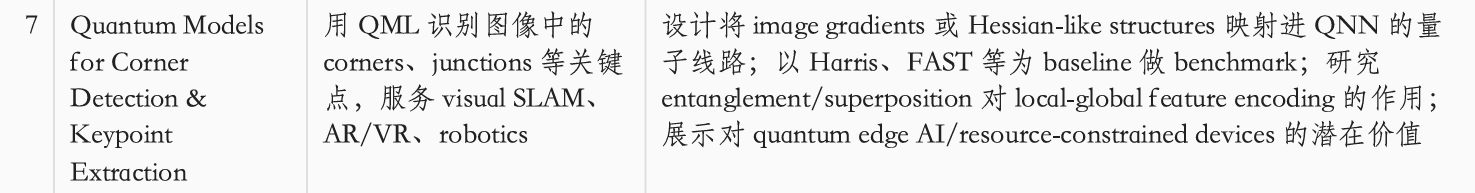
\includegraphics[width=0.96\linewidth]{figures/topic7.png}
    \caption{Hackathon 题目 7 的原始任务描述：用 QML 识别图像中的 corners、junctions 等关键点，并和 Harris、FAST 等方法对比。}
\end{figure}

已有 QNN 搭建计划书定义了 patch-level 二分类接口：输入候选点 $p$ 的局部特征向量 $x_p$，输出 $p_{\rm corner}(p)\in[0,1]$。第一版推荐五维特征
\begin{equation}
    x_p=[I_x(p),I_y(p),\lambda_1(p),\lambda_2(p),R(p)],
\end{equation}
其中 $R(p)=\det M(p)-k\Tr(M(p))^2$ 是 Harris response，$M(p)$ 是局部窗口 structure tensor。原计划书也已经给出了 feature normalization、angle encoding、data re-uploading、$R_zR_yR_z$ 变分层、纠缠层、Pauli-$Z$ 测量和线性 readout 的模块化实现路径。

本计划书是在该五量子比特方案上的“低维压缩与 QPP 理论化”版本：保留局部梯度结构特征和 data re-uploading 思想，但把短期主模型聚焦到 1--2 qubit，使项目更适合 hackathon 展示。

\section{理论基础：单量子比特 QNN 为什么能学习一元解析函数}

\subsection{Data re-uploading QNN 的基本形式}

一元输入 $x\in[-\pi,\pi]$ 的单量子比特 data re-uploading QNN 可写成
\begin{equation}
    U_\Theta(x)
    = W_L(\theta_L) E(x) W_{L-1}(\theta_{L-1})E(x)\cdots W_1(\theta_1)E(x)W_0(\theta_0),
\end{equation}
其中 $E(x)$ 是 encoding block，例如 $R_z(x)$ 或 $R_y(x)R_z(x)$，$W_\ell(\theta_\ell)$ 是可训练的单量子比特旋转，例如
\begin{equation}
    W_\ell(\theta_\ell)=R_z(\alpha_\ell)R_y(\beta_\ell)R_z(\gamma_\ell).
\end{equation}
模型输出通常是某个 Pauli observable 的期望值：
\begin{equation}
    g_\Theta(x)=\langle 0|U_\Theta(x)^\dagger Z U_\Theta(x)|0\rangle.
\end{equation}

\subsection{Fourier/Laurent 多项式视角}

考虑 $E(x)=R_z(x)$，有
\begin{equation}
    R_z(x)=\begin{pmatrix}
        e^{-ix/2} & 0 \\
        0 & e^{ix/2}
    \end{pmatrix}.
\end{equation}
每次 re-uploading 都会向矩阵元引入 $e^{\pm ix/2}$ 因子。经过 $L$ 次数据重上传后，$U_\Theta(x)$ 的矩阵元是关于 $z=e^{ix/2}$ 的有限 Laurent 多项式。测量期望值 $g_\Theta(x)$ 则成为关于 $e^{ix}$ 的有限三角多项式：
\begin{equation}
    g_\Theta(x)=\sum_{k=-K}^{K} c_k e^{ikx},
    \qquad c_{-k}=c_k^*,
\end{equation}
其中频率上界 $K$ 与 re-uploading 层数成正比。

Yu、Yao、Li 和 Wang 在 single-qubit native QNN 的理论工作中证明，特定单量子比特 QNN 结构不仅“类似 Fourier 级数”，而且可以在满足有界性和 unitary completion 条件时实现目标三角多项式，并建立可训练旋转参数与 Fourier 系数之间的对应关系 \cite{yu2022singlequbit}。

\begin{theorem}[单量子比特 QNN 的一元函数逼近，非正式表述]
给定一元实值函数 $f:[-\pi,\pi]\to\mathbb{R}$，若 $f$ 经过适当缩放后有界于 $[-1,1]$，则可用有限 Fourier partial sum 近似 $f$；相应地，存在足够深的单量子比特 data re-uploading QNN，使其 Pauli-$Z$ 期望值 $g_\Theta(x)$ 以任意给定精度逼近 $f$ 的缩放版本。
\end{theorem}

\subsection{解析函数的资源缩放}

如果 $f$ 是 $2\pi$ 周期解析函数，并且可以解析延拓到实轴附近的复条带 $|\Im z|<\rho$，则 Fourier 系数通常满足指数衰减
\begin{equation}
    |c_k|\le C e^{-\rho |k|}.
\end{equation}
因此，截断到 $|k|\le K$ 的 Fourier partial sum 误差满足类似
\begin{equation}
    \|f-f_K\|\lesssim C' e^{-\rho K}.
\end{equation}
为了达到误差 $\epsilon$，只需
\begin{equation}
    K=O\!\left(\log\frac{1}{\epsilon}\right).
\end{equation}
若 QNN 层数 $L$ 控制可生成频率 $K$，则解析函数的逼近层数对精度呈对数级增长。这就是“1-qubit QNN 可以模拟/逼近一元解析函数”这一叙事的核心数学来源。

\begin{warningbox}
严格讲，有限深度 QNN 精确实现的是有限三角多项式，而不是任意非多项式解析函数本身；“学习任意解析函数”应理解为在紧区间上、经过输出幅度归一化后以任意精度逼近。此外，该结论是表达能力结论，不保证随机初始化和梯度训练一定能高效找到对应参数。
\end{warningbox}

\section{Quantum Phase Processing 简介与本项目如何借用它}

Quantum Phase Processing (QPP) 是一种对酉算符本征相位直接施加函数变换的算法框架。若
\begin{equation}
    U=\sum_j e^{i\tau_j}|\chi_j\rangle\langle\chi_j|,
\end{equation}
QPP 通过单量子比特旋转和 controlled-$U$ 组成的线路，使 ancilla 在每个本征态子空间中经历一个依赖相位 $\tau_j$ 的单量子比特变换。形式上，QPP 线路可以分解为
\begin{equation}
    \bigoplus_j W_\Theta(\tau_j),
\end{equation}
其中 $W_\Theta(\tau)$ 是一个单量子比特相位处理线路。通过设计旋转角 $\Theta$，可让 ancilla 的测量期望值或振幅实现目标三角多项式 $F(\tau)$。Wang、Zhang、Yu 和 Wang 的 QPP 工作展示了这一框架在相位估计、Hamiltonian simulation、entropy estimation 等任务中的应用 \cite{wang2023qpp}。

本项目不需要真的构造高维 controlled-$U$，也不主张图像 patch 本身就是量子本征态。我们借用 QPP 的两点思想：
\begin{enumerate}[leftmargin=2.0em]
    \item \textbf{相位/角度是函数处理的载体。} 将局部图像特征归一化为旋转角 $\phi$，再通过 $R_z(\phi)$、$R_y(\phi)$ 和可训练旋转形成可学习三角多项式。
    \item \textbf{一个 ancilla 或极少 qubit 可以成为紧凑的非线性 Fourier 处理器。} 对一维 cornerness score $t$，1-qubit QNN 可以直接作为 QPP-style phase processor；对二维局部结构特征，2-qubit data re-uploading QNN 则作为多变量扩展 ansatz。
\end{enumerate}

\section{角点/交叉点的低维特征设计}

\subsection{Structure tensor 与 Harris 几何}

给定灰度图 $I(x,y)$，先用 Sobel、Scharr 或 Gaussian derivative 得到一阶梯度 $I_x,I_y$。以候选点 $p=(x_0,y_0)$ 为中心的局部窗口 $W$ 上定义
$g_x(u,v)=I_x(x_0+u,y_0+v)$ 与 $g_y(u,v)=I_y(x_0+u,y_0+v)$，则 structure tensor 为
\begin{equation}
M(p)=\sum_{(u,v)\in W} w(u,v)
\begin{pmatrix}
g_x(u,v)^2 & g_x(u,v)g_y(u,v)\\
g_x(u,v)g_y(u,v) & g_y(u,v)^2
\end{pmatrix}.
\end{equation}
其中 $w(u,v)$ 通常取 Gaussian window。记 $M(p)$ 的特征值为
\begin{equation}
    \lambda_1(p)\ge \lambda_2(p)\ge 0.
\end{equation}
Harris response 定义为
\begin{equation}
    R(p)=\det M(p)-k\Tr(M(p))^2
    =\lambda_1\lambda_2-k(\lambda_1+\lambda_2)^2.
\end{equation}
经典角点判据的几何解释是：平坦区域 $\lambda_1\approx\lambda_2\approx 0$；边缘区域 $\lambda_1\gg\lambda_2\approx0$；角点或交叉区域 $\lambda_1$ 与 $\lambda_2$ 都不小。

\subsection{为什么不把 $[I_x,I_y]$ 作为唯一主特征}

中心点梯度
\begin{equation}
    x_p^{\rm raw}=[I_x(p),I_y(p)]
\end{equation}
只描述一个像素附近的一阶变化方向，不能表达局部窗口内是否存在多个方向的结构。对交叉线条或 blob-like junction，中心处由于对称性可能 $I_x\approx I_y\approx 0$；对单边缘中心，梯度可能较大但只有一个方向；对噪声点，梯度也可能偶然较大。因此 $[I_x,I_y]$ 是重要消融项，但不是最稳健的主输入。

\subsection{推荐的二维主特征}

\paragraph{特征组 B：structure eigenvalues.}
\begin{equation}
    x_p^{(B)}=[\lambda_1(p),\lambda_2(p)].
\end{equation}
优点是信息直接、旋转不变、和 Harris/Shi-Tomasi 经典判据紧密相关。缺点是尺度可能跨度较大，需要 log 或 robust normalization。

\paragraph{特征组 C：energy + isotropy.}
\begin{equation}
    S(p)=\lambda_1(p)+\lambda_2(p),
\end{equation}
\begin{equation}
    \eta(p)=\frac{4\lambda_1(p)\lambda_2(p)}{(\lambda_1(p)+\lambda_2(p)+\epsilon)^2}.
\end{equation}
这里 $S$ 表示局部结构强度，$\eta\in[0,1]$ 表示二方向性或各向同性。平坦区 $S$ 小；单边缘 $S$ 可能大但 $\eta$ 小；角点/交叉点 $S$ 大且 $\eta$ 大。该特征组对“是否存在两个显著方向”有更强解释性。

\paragraph{一维 scalar cornerness.}
为了使用理论最干净的 1-qubit QPP-style 模型，可以进一步把二维结构压缩成一个标量 $t$：
\begin{equation}
    t_{c,\epsilon}(p)=\operatorname{norm}\left(\log(S(p)+\epsilon)+c\,\eta(p)\right),
\end{equation}
或
\begin{equation}
    t_{\epsilon}(p)=\operatorname{norm}\left(\log(\lambda_2(p)+\epsilon)\right),
\end{equation}
其中 $c$ 控制对二维性的奖励强度，$\epsilon$ 控制低能量区域的数值稳定性。短期实验可对 $c\in\{0.25,0.5,1,2,4\}$、$\epsilon\in\{10^{-8},10^{-6},10^{-4},10^{-3}\}$ 做验证集搜索；更进一步可将 $c$ 设为可训练参数。

\subsection{特征归一化与角度映射}

对每一维特征 $x_j$，使用训练集统计量标准化：
\begin{equation}
    z_j=\frac{x_j-\mu_j}{\sigma_j+\epsilon_{\rm std}}.
\end{equation}
然后进行截断：
\begin{equation}
    z_j\leftarrow \clip(z_j,-3,3),
\end{equation}
再映射为量子旋转角：
\begin{equation}
    \phi_j=\frac{\pi}{3} z_j,
    \qquad \phi_j\in[-\pi,\pi].
\end{equation}
该映射与原五量子比特计划书一致，优点是数值稳定、可复现、不会因少数异常梯度导致旋转角过大。

\section{主电路模型一：二维结构特征的 2-qubit QNN}

\subsection{输入选择}

2-qubit 主模型使用两个 qubit 分别承载两个局部结构特征。推荐两套默认配置：
\begin{align}
    \text{2q-}\lambda: \quad & [\phi_0,\phi_1] = \operatorname{AngleMap}([\lambda_1,\lambda_2]),\\
    \text{2q-}S\eta: \quad & [\phi_0,\phi_1] = \operatorname{AngleMap}([\log(S+\epsilon),\eta]).
\end{align}
$\lambda$ 版本更贴近 classical cornerness；$S\eta$ 版本更有解释性，更便于展示“强度 + 二维性”的判定逻辑。

\subsection{线路定义}

令初态为 $|00\rangle$。$L$ 层 data re-uploading 线路定义为
\begin{equation}
    |\psi_p\rangle = U^{(2q)}_\Theta(\bm\phi_p)|00\rangle,
\end{equation}
其中
\begin{equation}
    U^{(2q)}_\Theta(\bm\phi)=\prod_{\ell=1}^{L}
    U_{\rm ent}U_{{\rm var},\ell}(\Theta_\ell)U_{\rm enc}(\bm\phi).
\end{equation}
实际作用顺序为 encoding $\rightarrow$ trainable rotations $\rightarrow$ entanglement。

编码层为
\begin{equation}
    U_{\rm enc}(\bm\phi)=\prod_{j=0}^{1} R_y^{(j)}(\phi_j)R_z^{(j)}(\phi_j).
\end{equation}
变分层为
\begin{equation}
    U_{{\rm var},\ell}(\Theta_\ell)=\prod_{j=0}^{1}
    R_z^{(j)}(\alpha_{\ell j})R_y^{(j)}(\beta_{\ell j})R_z^{(j)}(\gamma_{\ell j}).
\end{equation}
纠缠层采用双向 CNOT：
\begin{equation}
    U_{\rm ent}=\operatorname{CNOT}_{0,1}\operatorname{CNOT}_{1,0},
\end{equation}
也可消融为 single CNOT、linear、none。

\begin{figure}[H]
\centering
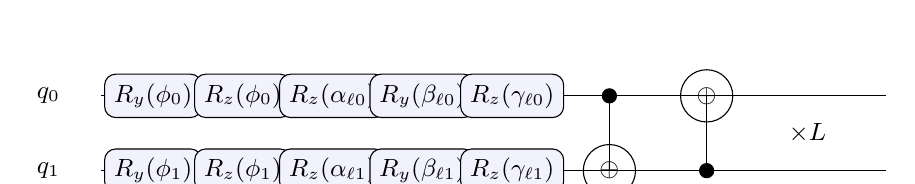
\begin{tikzpicture}[scale=0.95, every node/.style={font=\small}, gate/.style={draw,rounded corners,minimum width=1.0cm,minimum height=0.55cm,fill=blue!5}, var/.style={draw,rounded corners,minimum width=1.15cm,minimum height=0.55cm,fill=orange!10}, ent/.style={draw,rounded corners,minimum width=1.05cm,minimum height=0.55cm,fill=green!10}]
    \node at (-0.7,0) {$q_0$};
    \node at (-0.7,-1.0) {$q_1$};
    \draw[-] (0,0) -- (10.5,0);
    \draw[-] (0,-1.0) -- (10.5,-1.0);

    \foreach \x/\lab in {0.7/$R_y(\phi_0)$,1.9/$R_z(\phi_0)$,3.1/$R_z(\alpha_{\ell0})$,4.3/$R_y(\beta_{\ell0})$,5.5/$R_z(\gamma_{\ell0})$}{
      \node[gate] at (\x,0) {\lab};
    }
    \foreach \x/\lab in {0.7/$R_y(\phi_1)$,1.9/$R_z(\phi_1)$,3.1/$R_z(\alpha_{\ell1})$,4.3/$R_y(\beta_{\ell1})$,5.5/$R_z(\gamma_{\ell1})$}{
      \node[gate] at (\x,-1.0) {\lab};
    }
    \node[draw, circle, inner sep=1.8pt, fill=black] at (6.8,0) {};
    \node[draw, circle, minimum size=0.35cm] at (6.8,-1.0) {$\oplus$};
    \draw (6.8,0) -- (6.8,-1.0);
    \node[draw, circle, inner sep=1.8pt, fill=black] at (8.1,-1.0) {};
    \node[draw, circle, minimum size=0.35cm] at (8.1,0) {$\oplus$};
    \draw (8.1,0) -- (8.1,-1.0);
    \node at (9.45,-0.5) {$\times L$};
\end{tikzpicture}
\caption{2-qubit, one-layer block. 同一输入 $\bm\phi$ 在每一层重新上传。}
\end{figure}

\subsection{Readout 与分类概率}

测量
\begin{equation}
    z_0=\langle Z_0\rangle,
    \qquad z_1=\langle Z_1\rangle,
    \qquad z_{01}=\langle Z_0Z_1\rangle.
\end{equation}
输出 logit 为
\begin{equation}
    s(p)=b+w_0 z_0+w_1 z_1+w_{01}z_{01}.
\end{equation}
角点概率为
\begin{equation}
    p_{\rm corner}(p)=\sigma(s(p))=\frac{1}{1+e^{-s(p)}}.
\end{equation}
训练时推荐直接把 $s(p)$ 输入 \texttt{BCEWithLogitsLoss}，而不是在线路内部先做 sigmoid。

\subsection{参数量与推荐配置}

量子线路参数量为 $2\times 3\times L=6L$；若使用 $z_0,z_1,z_{01}$ readout，则经典 readout 参数为 4 个。默认 $L=3$ 时只有 18 个量子参数和 4 个经典 readout 参数。

\begin{table}[H]
\centering
\caption{2-qubit 主模型默认配置}
\begin{tabular}{lll}
\toprule
项目 & 默认值 & 消融选项 \\
\midrule
输入特征 & $[\lambda_1,\lambda_2]$ 或 $[\log(S+\epsilon),\eta]$ & $[I_x,I_y]$ \\
qubit 数 & 2 & 1, 3, 5 \\
re-uploading 层数 & $L=3$ & $L=1,2,4,6$ \\
encoding & $R_y(\phi)R_z(\phi)$ & only $R_y$, only $R_z$ \\
variational block & $R_zR_yR_z$ & $R_yR_z$, hardware-efficient \\
entanglement & bidirectional CNOT & none, single CNOT \\
measurement & $Z_0,Z_1,Z_0Z_1$ & $Z_0,Z_1$ only \\
loss & BCEWithLogitsLoss & focal loss, soft-label BCE \\
\bottomrule
\end{tabular}
\end{table}

\subsection{表达能力解释}

每一层 encoding 都把 $e^{\pm i\phi_0}$、$e^{\pm i\phi_1}$ 类型的相位因子注入量子态。可训练旋转和纠缠门将这些频率分量混合。经过 $L$ 层后，测量期望值可以看成一个有限阶二元三角多项式 ansatz：
\begin{equation}
    g_\Theta(\phi_0,\phi_1)
    \approx \sum_{|k_0|,|k_1|\le K(L)} c_{k_0,k_1}
    e^{i(k_0\phi_0+k_1\phi_1)}.
\end{equation}
这使模型能够学习非线性、非轴对齐的二维判定边界。$Z_0Z_1$ readout 进一步提供类似交互项的观测，使“两个条件同时满足”的 corner 判定更自然。

该二元 ansatz 的理论严格性弱于一元 QPP/QNN 定理，因此在报告中应表述为“QPP-inspired multivariate data-reuploading ansatz”，而不是直接声称已经拥有完整 QPP 的任意二元函数合成定理。

\section{主电路模型二：1-qubit QPP-style QNN}

1-qubit 方案有两个互补版本。前者理论最干净，后者保留两个原始结构特征。

\subsection{版本 A：单一 cornerness 标量 $t$ 的 QPP-style QNN}

先通过经典可解释 scalarizer 把局部结构压缩成一维角度：
\begin{equation}
    t(p)=\operatorname{AngleMap}\left(\log(S(p)+\epsilon)+c\eta(p)\right).
\end{equation}
然后使用单量子比特线路
\begin{equation}
    U^{(1q,t)}_\Theta(t)=\prod_{\ell=1}^{L}
    R_z(t)R_y(a_\ell)R_z(b_\ell),
\end{equation}
或更对称地
\begin{equation}
    U^{(1q,t)}_\Theta(t)=\prod_{\ell=1}^{L}
    R_z(t)R_z(\alpha_\ell)R_y(\beta_\ell)R_z(\gamma_\ell).
\end{equation}
测量
\begin{equation}
    z=\langle Z\rangle,
    \qquad s(p)=wz+b,
    \qquad p_{\rm corner}(p)=\sigma(s(p)).
\end{equation}

该版本可直接对接一元 QNN 的 Fourier 理论：$s(p)$ 是 $t$ 的可训练三角多项式再经过 sigmoid 得到的 soft classification function。它适合在 hackathon 中展示“一个 qubit 的解析函数学习能力如何落地到局部 cornerness 判定”。

\paragraph{关于 $c$、$\epsilon$ 和 $L$ 的调参。}
$c$ 和 $\epsilon$ 不应固定后就不再讨论。推荐如下策略：
\begin{enumerate}[leftmargin=2.0em]
    \item 先设 $\epsilon$ 为训练集 $S$ 的 $10^{-4}$ 分位或固定 $10^{-8}$，保证 $\log(S+\epsilon)$ 稳定。
    \item 对 $c\in\{0,0.25,0.5,1,2,4,8\}$ 网格搜索，验证集 PR-AUC 选优。
    \item 对 $L\in\{2,3,4,6,8\}$ 搜索，画出 PR-AUC/F1 与参数量曲线。
    \item 第二版把 $c=\softplus(\rho)$ 设为可训练参数，和 QNN 参数联合训练；或定义 $t=a\,\operatorname{std}(\log S)+b\,\operatorname{std}(\eta)+d$，其中 $a,b,d$ 可训练。
\end{enumerate}

\subsection{版本 B：two-feature interleaved 1-qubit QNN}

若不希望先把二维特征手动压缩为 $t$，可使用单量子比特交替编码两个角度：
\begin{equation}
    U^{(1q,2f)}_\Theta(\phi_0,\phi_1)
    =\prod_{\ell=1}^{L}
    R_z(\phi_0)R_y(a_\ell)R_z(\phi_1)R_y(b_\ell)R_z(c_\ell).
\end{equation}
由于 $R_z(\phi_0)$ 和 $R_z(\phi_1)$ 被可训练 $R_y$ 隔开，二者不会简单合并为 $R_z(\phi_0+\phi_1)$，输出可以包含两个输入的非线性混合。

该版本的优势是 qubit 数仍为 1，同时保留两个结构特征；劣势是理论叙事比 scalar $t$ 版本弱一些，应称为 data-reuploading universal classifier 风格的 1-qubit ansatz。

\begin{figure}[H]
\centering
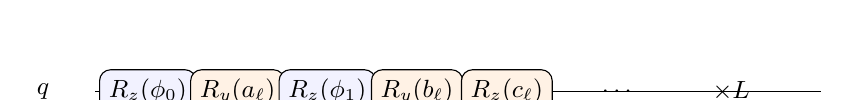
\begin{tikzpicture}[scale=0.95, every node/.style={font=\small}, gate/.style={draw,rounded corners,minimum width=1.0cm,minimum height=0.55cm,fill=blue!5}, var/.style={draw,rounded corners,minimum width=1.0cm,minimum height=0.55cm,fill=orange!10}]
    \node at (-0.7,0) {$q$};
    \draw[-] (0,0) -- (9.7,0);
    \foreach \x/\lab/\style in {0.7/$R_z(\phi_0)$/gate,1.9/$R_y(a_\ell)$/var,3.1/$R_z(\phi_1)$/gate,4.3/$R_y(b_\ell)$/var,5.5/$R_z(c_\ell)$/var}{
      \node[\style] at (\x,0) {\lab};
    }
    \node at (7.0,0) {$\cdots$};
    \node at (8.5,0) {$\times L$};
\end{tikzpicture}
\caption{1-qubit two-feature interleaved QNN block.}
\end{figure}

\section{数据集构造与训练流程}

\subsection{样本构造}

对每张训练图像，执行以下步骤：
\begin{enumerate}[leftmargin=2.0em]
    \item 灰度化并进行轻度 Gaussian smoothing，减小噪声对梯度的影响。
    \item 用 Sobel、Scharr 或 Gaussian derivative 计算 $I_x,I_y$。
    \item 对每个候选中心点 $p$，计算局部 structure tensor $M(p)$、特征值 $\lambda_1,\lambda_2$、$R$、$S$、$\eta$。
    \item 根据人工标注或 synthetic generator 的 ground truth 生成标签。距离真实 corner/junction 小于 $r_{\rm pos}$ 的候选点作为 positive；距离所有正点大于 $r_{\rm neg}$ 的点作为 negative；中间灰区不训练，以降低 label noise。
    \item 负样本按区域分层采样：平坦区、单边缘、非中心交叉、纹理噪声都要覆盖。
\end{enumerate}

\subsection{训练/验证/测试划分}

建议按图像而不是按像素随机切分，避免同一张图中的相邻 patch 同时出现在训练和测试中造成泄漏。synthetic toy 可以使用 stratified split；真实图像应采用 image-level split 或 scene-level split。

\subsection{损失函数与优化器}

使用 logits 形式的 weighted binary cross entropy：
\begin{equation}
    \mathcal{L}=-\frac{1}{N}\sum_{i=1}^N \left[\alpha y_i\log\sigma(s_i)+(1-y_i)\log(1-\sigma(s_i))\right],
\end{equation}
或直接在 PyTorch 中使用
\begin{equation}
    \texttt{BCEWithLogitsLoss(pos\_weight=\#neg/\#pos)}.
\end{equation}
优化器使用 Adam。模拟器第一版用 exact expectation，不加入 shot noise；第二版可加入 1024 或 2048 shots 估计测量噪声。

\subsection{推荐训练超参数}

\begin{table}[H]
\centering
\caption{第一阶段推荐超参数}
\begin{tabular}{lll}
\toprule
项目 & 2q-QNN 默认值 & 1q-QNN 默认值 \\
\midrule
输入 & $[\lambda_1,\lambda_2]$ 或 $[S,\eta]$ & $t$ 或 interleaved $[S,\eta]$ \\
层数 & $L=3$ & $L=4$，再扫 $2,3,6,8$ \\
encoding & $R_yR_z$ & $R_z$ phase encoding \\
readout & $Z_0,Z_1,Z_0Z_1$ + linear & $Z$ + affine \\
optimizer & Adam & Adam \\
learning rate & $10^{-3}$--$5\times10^{-2}$ & $10^{-3}$--$5\times10^{-2}$ \\
batch size & 32, 64, 128 & 32, 64, 128 \\
epochs & 50--200 & 50--300 \\
shots & exact first & exact first \\
metric for selection & PR-AUC, F1 & PR-AUC, F1 \\
\bottomrule
\end{tabular}
\end{table}

\subsection{整图应用流程}

训练得到模型后，对一张完整图像执行：
\begin{enumerate}[leftmargin=2.0em]
    \item 计算每个像素或稀疏候选点的二维结构特征。
    \item 使用训练阶段保存的 normalizer 映射到角度 $\bm\phi(p)$。
    \item 对每个 $p$ 运行 QNN 得到 $p_{\rm corner}(p)$。
    \item 将概率写回图像坐标形成 heatmap。
    \item 对 heatmap 做 threshold 和 NMS，得到离散 keypoints。
    \item 计算 patch-level 和 keypoint-level 指标，并和经典算法的 heatmap 或 score map 对齐比较。
\end{enumerate}

\section{与经典算法的全面对比设计}

\subsection{低层角点检测 baseline}

\begin{enumerate}[leftmargin=2.0em]
    \item \textbf{Harris threshold.} 使用 $R=\det M-k\Tr(M)^2$，阈值由验证集选择。Harris 和 Stephens 的原始工作把局部自相关矩阵用于 combined corner and edge detector，是本项目 structure tensor 特征的直接经典基线 \cite{harris1988combined}。
    \item \textbf{Shi-Tomasi / min eigenvalue.} 使用 $\min(\lambda_1,\lambda_2)=\lambda_2$ 作为 cornerness score。
    \item \textbf{FAST.} 使用 accelerated segment test 作为实时角点检测 baseline。Rosten 和 Drummond 的 FAST 工作展示了机器学习导出的高速角点检测器，并强调实时 tracking 应用 \cite{rosten2006fast}。
    \item \textbf{DoG/SIFT detector 或 LoG.} 作为尺度空间 keypoint detector baseline，若时间允许加入。
\end{enumerate}

\subsection{同特征 classical ML baseline}

为了公平比较 QNN 的非线性 readout 能力，必须使用相同输入特征训练经典模型：
\begin{enumerate}[leftmargin=2.0em]
    \item logistic regression: 检查二维特征是否线性可分；
    \item SVM/RBF 或 kernel logistic: 检查经典核方法上限；
    \item small MLP: 例如 2-8-1 或 2-16-8-1；
    \item random forest / gradient boosting: 检查 tabular feature 的强基线；
    \item QNN without re-uploading / without entanglement: 检查量子结构中的关键组件。
\end{enumerate}

若 QNN 不能超过相同特征下的小型 MLP，则不应声称性能优势；可以转而强调“few-qubit compact nonlinear classifier 的可解释结构与相位处理机制”。

\subsection{评价指标}

patch-level 指标：accuracy、precision、recall、F1、ROC-AUC、PR-AUC。由于角点样本稀少，PR-AUC 和 F1 优先于 accuracy。

keypoint-level 指标：repeatability、localization error、matching score、检测点数量、RANSAC inlier ratio。短期项目可以先报告 patch-level，再展示 qualitative heatmap 和 NMS 后的 keypoint overlay。

\section{Toy sanity check：检查了什么，结果说明什么}

\subsection{toy 数据生成}

初步 toy check 使用合成的 $48\times48$ blurred line patches。正样本是两条线在中心附近交叉；负样本包括三类：穿过中心的单线、远离中心的交叉、平坦或噪声背景。每个 patch 提取以下特征：中心梯度 $I_x,I_y$、structure tensor 特征值 $\lambda_1,\lambda_2$、Harris response、$S=\lambda_1+\lambda_2$、$\eta$。

这个 toy 的目的不是证明真实图像性能，而是做三个 sanity checks：
\begin{enumerate}[leftmargin=2.0em]
    \item 检查中心 $[I_x,I_y]$ 是否真的信息不足；
    \item 检查 $[\lambda_1,\lambda_2]$ 与 $[S,\eta]$ 是否更适合表示角点/交叉点；
    \item 检查 2q-QNN $L=3$ 和 1q-QNN $L=4$ 是否能在小样本低维特征上训练成功。
\end{enumerate}

\begin{figure}[H]
    \centering
    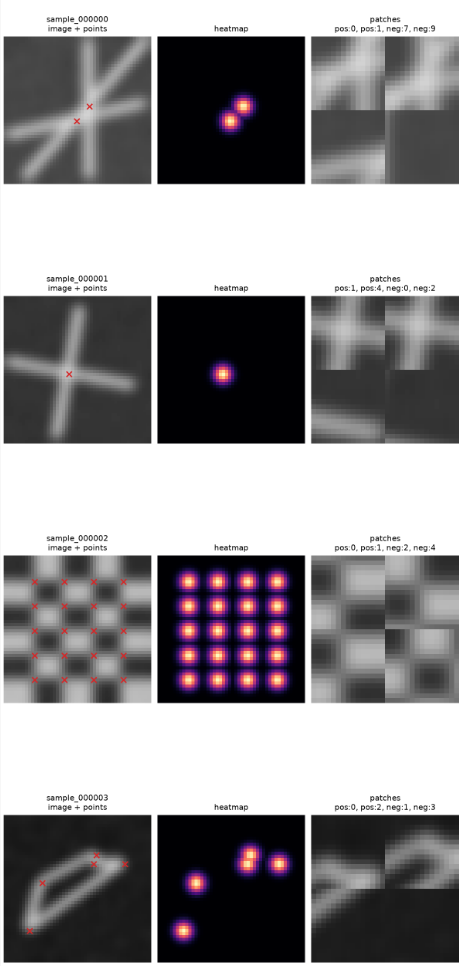
\includegraphics[width=0.48\linewidth]{figures/toy_examples.png}
    \caption{toy 数据示例。左列为合成 patch 和标注点，中列为目标 heatmap，右列为正负 patch 样本示意。}
\end{figure}

\subsection{toy 结果}

\begin{table}[H]
\centering
\caption{toy sanity check 初步结果。数据规模较小，仅用于方向验证。}
\resizebox{\linewidth}{!}{%
\begin{tabular}{llrrrrrr}
\toprule
输入特征 & 模型 & Acc & F1 & PR-AUC & ROC-AUC & Precision & Recall \\
\midrule
$[I_x,I_y]$ & Logistic & 0.472 & 0.513 & 0.471 & 0.677 & 0.370 & 0.833 \\
$[I_x,I_y]$ & 2q-QNN, $L=3$ & 0.639 & 0.606 & 0.530 & 0.747 & 0.476 & 0.833 \\
$[I_x,I_y]$ & 1q-QNN, $L=4$ & 0.667 & 0.667 & 0.739 & 0.840 & 0.500 & 1.000 \\
\midrule
$[\lambda_1,\lambda_2]$ & Logistic & 0.972 & 0.957 & 1.000 & 1.000 & 1.000 & 0.917 \\
$[\lambda_1,\lambda_2]$ & 2q-QNN, $L=3$ & 1.000 & 1.000 & 1.000 & 1.000 & 1.000 & 1.000 \\
$[\lambda_1,\lambda_2]$ & 1q-QNN, $L=4$ & 0.778 & 0.667 & 0.790 & 0.826 & 0.667 & 0.667 \\
\midrule
$[S,\eta]$ & Logistic & 0.889 & 0.818 & 0.936 & 0.955 & 0.900 & 0.750 \\
$[S,\eta]$ & 2q-QNN, $L=3$ & 0.917 & 0.857 & 0.959 & 0.972 & 1.000 & 0.750 \\
$[S,\eta]$ & 1q-QNN, $L=4$ & 0.722 & 0.643 & 0.744 & 0.816 & 0.562 & 0.750 \\
\bottomrule
\end{tabular}%
}
\end{table}

\subsection{结果解释}

初步结果与可行性判断一致。$[I_x,I_y]$ 上的模型表现明显不稳定，说明中心梯度不是可靠充分特征；$[\lambda_1,\lambda_2]$ 和 $[S,\eta]$ 明显更有判别力。2q-QNN, $L=3$ 在两个结构特征组上都取得了很高的 PR-AUC 和 F1，在 $[S,\eta]$ 上相对 logistic 有小幅提升。1q-QNN 在 raw gradient 上反而能学到一些非线性结构，但在结构特征上未达到 2q-QNN，提示单量子比特模型需要更细致地调节 scalarizer、层数、初始化和 readout。

\begin{warningbox}
该 toy 结果不能外推为真实图像性能结论。它只说明：二维结构特征是更合理的主输入；few-qubit QNN 可以在该低维任务上训练；2q-QNN $L=3$ 是一个值得作为主线推进的短期模型。
\end{warningbox}

\section{消融实验矩阵}

\subsection{输入特征消融}

\begin{longtable}{p{0.07\linewidth}p{0.37\linewidth}p{0.48\linewidth}}
\caption{输入特征消融设计}\\
\toprule
编号 & 特征 & 目的 \\
\midrule
A & $[I_x,I_y]$ & 验证中心梯度是否不足，作为反例/低信息基线 \\
B & $[\lambda_1,\lambda_2]$ & 结构张量 eigenvalue 主模型 \\
C & $[\log(S+\epsilon),\eta]$ & 强度 + 二维性，可解释主模型 \\
D & $[\lambda_2,R]$ & 与 Shi-Tomasi/Harris score 对齐 \\
E & $[I_x,I_y,\lambda_1,\lambda_2,R]$ & 原计划书五维完整特征 \\
F & $[I_x,I_y,I_x^2,I_y^2,I_xI_y,\lambda_1,\lambda_2,R]$ & 八维扩展 \\
G & Hessian features $[I_{xx},I_{xy},I_{yy},\det H,\Tr H]$ & 纹理和曲率增强 \\
\bottomrule
\end{longtable}

\subsection{量子线路消融}

\begin{table}[H]
\centering
\caption{量子线路消融设计}
\begin{tabular}{p{0.18\linewidth}p{0.35\linewidth}p{0.37\linewidth}}
\toprule
因素 & 取值 & 观察问题 \\
\midrule
qubit 数 & 1, 2, 5 & qubit 数与特征维度/表达能力的 trade-off \\
层数 $L$ & 1, 2, 3, 4, 6, 8 & data re-uploading 是否提升 Fourier 频率容量 \\
encoding & $R_y$, $R_z$, $R_yR_z$ & 相位编码是否有实际增益 \\
entanglement & none, CNOT$_{0,1}$, bidirectional CNOT & 交互项是否需要纠缠 \\
readout & $Z$ only, all $Z$, $Z_iZ_j$ included & classical readout 是否限制输出 \\
shots & exact, 1024, 2048 & shot noise 下鲁棒性 \\
noise & none, depolarizing, amplitude damping & NISQ 噪声敏感性 \\
\bottomrule
\end{tabular}
\end{table}

\section{实现模块建议}

\subsection{代码结构}

建议代码目录如下：
\begin{lstlisting}
qpp_corner_qnn/
  preprocessing.py        # gradients, structure tensor, normalizer
  features.py             # feature sets A/B/C/D/E/F/G
  qnn_circuits.py          # 1q and 2q QNN modules
  classical_baselines.py   # Harris, FAST, logistic, MLP, SVM
  train.py                # training loop
  evaluate.py             # patch/keypoint metrics
  infer_heatmap.py         # whole-image heatmap + NMS
  run_ablation.py          # experiment grid
  configs/
    twoq_lambda_L3.yaml
    twoq_seta_L3.yaml
    oneq_scalar_L4.yaml
  notebooks/
    visualize_toy.ipynb
    visualize_heatmap.ipynb
\end{lstlisting}

\subsection{核心训练伪代码}

\begin{lstlisting}[language=Python]
# X_raw: handcrafted local features, y: binary labels
normalizer.fit(X_train)
Phi_train = normalizer.transform_to_angles(X_train)
Phi_val   = normalizer.transform_to_angles(X_val)

model = TwoQubitReuploadQNN(n_layers=3,
                            encoding="ryrz",
                            entanglement="bidirectional_cnot",
                            readout="z0_z1_z01")
criterion = torch.nn.BCEWithLogitsLoss(pos_weight=num_neg / num_pos)
optimizer = torch.optim.Adam(model.parameters(), lr=lr)

for epoch in range(num_epochs):
    for Phi_batch, y_batch in loader:
        logits = model(Phi_batch)
        loss = criterion(logits, y_batch.float())
        optimizer.zero_grad()
        loss.backward()
        optimizer.step()

    val_prob = torch.sigmoid(model(Phi_val))
    report_pr_auc_f1(val_prob, y_val)
\end{lstlisting}

\section{后续优化方向}

\subsection{优化 1-qubit 模型}

1-qubit 模型的潜力主要取决于 scalarizer 和频率容量。后续重点包括：
\begin{enumerate}[leftmargin=2.0em]
    \item 将 $t=\log(S+\epsilon)+c\eta$ 改为 learnable scalarizer：
    \begin{equation}
        t=a\,\operatorname{std}(\log(S+\epsilon))+b\,\operatorname{std}(\eta)+d,
    \end{equation}
    其中 $a,b,d$ 与 QNN 参数联合训练。
    \item 使用 monotonic cornerness 约束，例如强制 $t$ 对 $S$ 与 $\eta$ 单调递增。
    \item 对 $L$ 做系统 sweep，并画出 PR-AUC vs. parameter count 曲线。
    \item 改进初始化：小角度初始化、Fourier coefficient inspired initialization、多随机种子 ensemble。
    \item 加入 $\langle X\rangle,\langle Y\rangle,\langle Z\rangle$ 多轴 readout，而不只测 $Z$。
\end{enumerate}

\subsection{增强 2-qubit 模型}

\begin{enumerate}[leftmargin=2.0em]
    \item 将 readout 扩展为 $Z_0,Z_1,Z_0Z_1,X_0,X_1$，检查是否提升分类边界。
    \item 使用 data scaling 参数：$R_y(a_j\phi_j)R_z(b_j\phi_j)$，其中 $a_j,b_j$ 可训练或网格搜索。
    \item 对 $[\lambda_1,\lambda_2]$ 使用 log transform：$[\log(\lambda_1+\epsilon),\log(\lambda_2+\epsilon)]$。
    \item 加入轻量 classical pre-readout：例如 normalizer 后的 affine transform 再输入 QNN。
    \item 在真实数据中加入旋转、亮度、噪声、模糊等 augmentation，检验泛化。
\end{enumerate}

\subsection{从 patch-level 到 keypoint-level}

短期先完成 patch-level 分类，下一步必须将模型输出转化为真实 keypoints：
\begin{enumerate}[leftmargin=2.0em]
    \item 用 QNN 输出整图 heatmap；
    \item threshold 由验证集选取，或控制固定 keypoint 数量；
    \item NMS 半径与标注容忍半径对齐；
    \item 评估 localization error 和 repeatability；
    \item 在 SLAM/匹配任务中测试 descriptor matching 和 RANSAC inlier ratio。
\end{enumerate}

\subsection{量子硬件/噪声叙事}

如果时间允许，可以加入 shot-noise 和 depolarizing-noise 模拟，展示低 qubit 数和低深度线路在 NISQ 约束下的潜在优势。这里的“优势”不是算法复杂度上的量子优势，而是硬件友好性和资源约束叙事：2 qubit、$L=3$、少量 CNOT、几十个参数，适合 edge AI / resource-constrained quantum device 的概念展示。

\section{Hackathon 主叙事}

建议最终展示叙事如下：

\begin{quote}
我们把角点检测重新表述为“局部几何相位处理”问题。传统 Harris/FAST 通过手工规则从局部梯度结构中产生 cornerness score；我们保留可解释的局部 structure tensor 特征，但用 QPP-inspired data-reuploading QNN 学习一个紧凑的非线性 Fourier decision surface。对于一维 cornerness score，单量子比特 QNN 具有清晰的 Fourier/解析函数逼近理论；对于二维结构特征，2-qubit QNN 通过数据重上传和纠缠学习 $[\lambda_1,\lambda_2]$ 或 $[S,\eta]$ 上的 smooth classification boundary。该方案只需 1--2 个 qubit，却能输出整图角点 heatmap，并可和 Harris、FAST、logistic regression、MLP 做透明对比。
\end{quote}

\subsection{短期可交付成果}

\begin{enumerate}[leftmargin=2.0em]
    \item 一个可运行的 synthetic toy demo，展示 patch、标签 heatmap、QNN heatmap；
    \item 2q-QNN $L=3$ 在 $[\lambda_1,\lambda_2]$ 和 $[S,\eta]$ 上的训练与评测；
    \item 1q-QNN scalar $t$ 与 interleaved two-feature 两个版本；
    \item Harris、FAST、logistic、MLP baseline；
    \item ablation 图：features、layers、encoding、entanglement、readout；
    \item 一页理论图：single-qubit QNN $\leftrightarrow$ Fourier series $\leftrightarrow$ analytic function approximation $\leftrightarrow$ QPP phase processing；
    \item 一页应用图：image $\rightarrow$ gradients $\rightarrow$ structure tensor $\rightarrow$ QNN $\rightarrow$ heatmap $\rightarrow$ NMS keypoints。
\end{enumerate}

\subsection{建议的 5 天执行排期}

\begin{table}[H]
\centering
\caption{Hackathon 执行排期}
\begin{tabular}{p{0.14\linewidth}p{0.31\linewidth}p{0.45\linewidth}}
\toprule
时间 & 目标 & 产出 \\
\midrule
Day 1 & synthetic generator + features & patch/heatmap 可视化，Harris/logistic baseline \\
Day 2 & 2q-QNN exact simulator & $[\lambda_1,\lambda_2]$ 和 $[S,\eta]$ 初步结果 \\
Day 3 & 1q-QNN + scalarizer sweep & $c,\epsilon,L$ 曲线，模型对比表 \\
Day 4 & 真实/半真实图像推理 & 整图 heatmap、NMS keypoints、baseline overlay \\
Day 5 & ablation + slides & 主叙事、局限性、demo video、最终报告 \\
\bottomrule
\end{tabular}
\end{table}

\section{风险点与应对策略}

\begin{longtable}{p{0.28\linewidth}p{0.34\linewidth}p{0.30\linewidth}}
\caption{风险点与应对方案}\\
\toprule
风险 & 表现 & 应对 \\
\midrule
$[I_x,I_y]$ 信息不足 & 模型无法泛化，heatmap 响应噪声大 & 把 $[I_x,I_y]$ 降级为消融，主模型使用 $[\lambda_1,\lambda_2]$ 或 $[S,\eta]$ \\
QNN 不超过 MLP & 性能 claim 受限 & 强调 compact quantum ansatz、QPP theory-inspired、资源约束展示；透明报告负结果 \\
正负样本不平衡 & accuracy 高但 recall 低 & 使用 pos\_weight、PR-AUC、hard negative mining \\
真实图像 label noise & 训练不稳定 & 使用 soft heatmap label，中间灰区不训练 \\
1q 模型表现弱 & F1/PR-AUC 低于 2q & scalarizer sweep、learnable scalarizer、多轴 readout、增加 $L$ \\
线路模拟慢 & ablation 跑不完 & 优先 exact statevector + small batch；先跑 1q/2q；5q 作为扩展 \\
\bottomrule
\end{longtable}

\section{结论}

该短期项目的可行路径非常明确：用 structure tensor 把局部几何压缩为 $[\lambda_1,\lambda_2]$ 或 $[S,\eta]$，再用 2-qubit $L=3$ data-reuploading QNN 作为主模型，输出角点/交叉点概率 heatmap；同时保留 1-qubit scalar $t$ QPP-style QNN 作为理论亮点模型。toy check 已初步显示二维结构特征明显优于中心梯度，2q-QNN 在合成交叉点任务上能够稳定训练并达到优良指标。后续重点是将 toy 扩展到更真实的图像、做完整消融、与 Harris/FAST/MLP 透明对比，并把“一个/两个 qubit 作为局部几何 Fourier decision processor”的叙事讲清楚。

\appendix
\section{附录：推荐报告中的 claim 写法}

\subsection{可以大胆说的内容}
\begin{enumerate}[leftmargin=2.0em]
    \item 单量子比特 data re-uploading QNN 对一元函数具有 Fourier/trigonometric polynomial 表达能力。
    \item 对周期解析函数，Fourier 系数指数衰减，因此低层数 QNN 有机会高效逼近平滑判定函数。
    \item 角点检测中的 structure tensor 特征天然是低维、可解释、rotation-invariant 的局部几何统计量。
    \item 2q-QNN $L=3$ 是一个资源很低的非线性分类器，可以输出角点 heatmap。
    \item toy sanity check 支持 $[\lambda_1,\lambda_2]$ 与 $[S,\eta]$ 是比 $[I_x,I_y]$ 更合理的二维输入。
\end{enumerate}

\subsection{需要避免的内容}
\begin{enumerate}[leftmargin=2.0em]
    \item 不说“量子优势已经被验证”。
    \item 不说“一个 qubit 从任意图像中识别任意角点”。
    \item 不说“中心梯度 $[I_x,I_y]$ 足够”。
    \item 不说“有限深度 QNN 精确表达任意 discontinuous binary indicator”。
    \item 不把 toy 结果包装成真实数据结论。
\end{enumerate}

\section{附录：参考文献中的关键作用}

Yu et al. \cite{yu2022singlequbit} 支撑“single-qubit native QNN 的 Fourier 表达能力与一元函数逼近”；Wang et al. \cite{wang2023qpp} 支撑“QPP 作为相位函数处理框架”；P\'erez-Salinas et al. \cite{perezsalinas2020data} 支撑“data re-uploading universal quantum classifier”；Harris and Stephens \cite{harris1988combined} 与 Rosten and Drummond \cite{rosten2006fast} 分别支撑经典角点检测 baseline。

\begin{thebibliography}{99}

\bibitem{yu2022singlequbit}
Zhan Yu, Hongshun Yao, Mujin Li, and Xin Wang.
\newblock Power and limitations of single-qubit native quantum neural networks.
\newblock \emph{Advances in Neural Information Processing Systems}, 35:27810--27823, 2022.
\newblock arXiv:2205.07848.

\bibitem{wang2023qpp}
Youle Wang, Lei Zhang, Zhan Yu, and Xin Wang.
\newblock Quantum phase processing and its applications in estimating phase and entropies.
\newblock \emph{Physical Review A}, 108:062413, 2023.
\newblock arXiv:2209.14278.

\bibitem{perezsalinas2020data}
Adri\'an P\'erez-Salinas, Alba Cervera-Lierta, Elies Gil-Fuster, and Jos\'e I. Latorre.
\newblock Data re-uploading for a universal quantum classifier.
\newblock \emph{Quantum}, 4:226, 2020.

\bibitem{harris1988combined}
Chris Harris and Mike Stephens.
\newblock A combined corner and edge detector.
\newblock In \emph{Alvey Vision Conference}, pages 147--151, 1988.

\bibitem{rosten2006fast}
Edward Rosten and Tom Drummond.
\newblock Machine learning for high-speed corner detection.
\newblock In \emph{European Conference on Computer Vision}, pages 430--443, 2006.

\bibitem{shi1994goodfeatures}
Jianbo Shi and Carlo Tomasi.
\newblock Good features to track.
\newblock In \emph{IEEE Conference on Computer Vision and Pattern Recognition}, pages 593--600, 1994.

\end{thebibliography}

\end{document}
